\documentclass{article}
\usepackage[utf8]{inputenc}

\documentclass{article}
\usepackage[utf8]{inputenc}
\usepackage{hyperref}
\usepackage[letterpaper, portrait, margin=1in]{geometry}
\usepackage{enumitem}
\usepackage{amsmath}
\usepackage{booktabs}
\usepackage{graphicx}

\usepackage{hyperref}
\hypersetup{
colorlinks=true,
    linkcolor=black,
    filecolor=black,      
    urlcolor=blue,
    citecolor=black,
}
\usepackage{natbib}

\usepackage{titlesec}
  
\title{Homework 4}
\author{Ioanna Maria Spyrou}
\date{Spring semester 2021}
  
\begin{document}
  
\maketitle


1.Yes, the trends were parallel before treatment and after treatment we notice a drop in pounds of bycatch on treated, which means that the program was efficient.See graph below:
\\
\begin{figure}[ht]
    \centering
    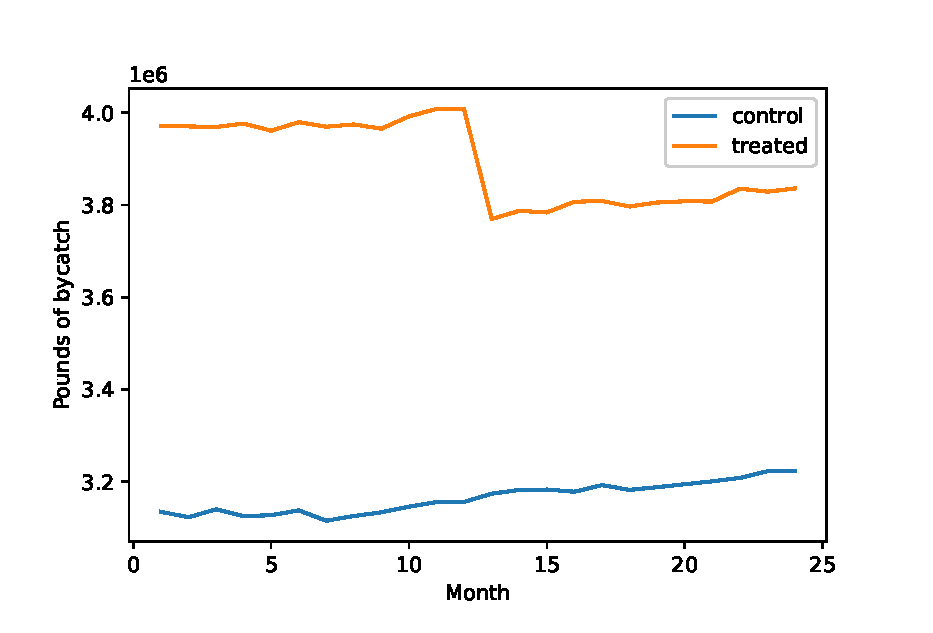
\includegraphics[scale = 0.7]{graph.eps}
    \caption{Bycatch for control and treated groups by month.}
    \label{fig:samplebars}
\end{figure}

2.The DID equals -8956.78, which mean that bycatch reduces by that amount due the program. So the estimator shows that the program worked.
\\
3.See table \ref{tab:coef_table}:

\begin{table}[ht]
    \centering
    \begin{tabular}{ll}
\toprule
{} & Coefficients \\
{} &       (s.e.) \\
\midrule
λ(t=2017)  &    137228.60 \\
           &   (18739.84) \\
a          &      2589.66 \\
           &    (-171.93) \\
g(i)       &      6406.37 \\
           &   (23343.87) \\
treat(i,t) &     -4406.11 \\
           &    (1860.59) \\
\bottomrule
\end{tabular}

    \caption{Sample regression coefficients table with standard errors.}
    \label{tab:coef_table}
\end{table}
\\ 
The result shows that if a firm is treated then bycatch reduces by 4406 pounds which is less than the amount estimated using sample analog on question 2.







\end{document}